\chapter{Kvantově inspirované evoluční algoritmy} \label{chapt:qiea}
Evoluční algoritmy, které vycházejí z principů kvantové mechaniky, se souhrnně označují jako kvantově inspirované evoluční algoritmy (\emph{Quantum Inspired Evolutionary Algorithms\,--\,QIEA}) a jsou navrženy především pro řešení optimalizačních problémů. 
Není však možné, aby tyto algoritmy využívaly všechny náležitosti vyplývající z kvantové mechaniky. 
Jedná se zejména o kvantové provázání, které nelze efektivně simulovat na klasických počítačích. 
Nicméně použití kvantově inspirované reprezentace v evolučních algoritmech se v některých případech ukázalo jako vhodný kompromis mezi průzkumem a exploatací, přičemž často umožňuje pracovat s menší populací jedinců, než by bylo nutné u klasických evolučních algoritmů~\cite{NaturalComputing}.

Tato kapitola nejdříve popíše, jak lze reprezentovat jedince v populaci, a následně se zaměří na dva způsoby transformace těchto jedinců pomocí kvantového rotačního hradla a~kvantové mutace. 
Poté charakterizuje následující kvantově inspirované evoluční algoritmy:
\begin{itemize}
    \item kvantově inspirovaný genetický algoritmus,
    \item kvantově inspirované simulované žíhání,
    \item kvantová evoluce roje a
    \item kvantově inspirovaná optimalizace rojem částic.
\end{itemize}
V poslední řadě jsou souhrnně vylíčeny zajímavé studie popisující situace, kde byly \emph{QIEA} využity. 

\section{Kódování řešení v kvantově inspirovaných evolučních algoritmech}
Jeden z možných způsobů reprezentace jedince v populaci v kvantově inspirovaných evolučních algoritmech vychází z konceptu kvantového bitu. 
Binární kvantově inspirované evoluční algoritmy využívají qubity k reprezentaci řešení, přičemž manipulace s nimi probíhá prostřednictvím kvantově inspirovaných operátorů~\cite{NaturalComputing}. 

V binárním kvantově inspirovaném evolučním algoritmu je qubit popsán dvojicí koeficientů $\alpha$ a~$\beta$, přičemž systém sestávající z $m$ qubitů lze zapsat v podobě matice jako: 
\begin{equation}\label{eq:quantum-representation}
    \begin{bmatrix}
        \alpha_1 & \alpha_2 & \dots & \alpha_m \\
        \beta_1  & \beta_2  & \dots & \beta_m
    \end{bmatrix},
\end{equation}
kde $\alpha_i,\beta_i \in \mathbb{R}$ a přičemž pro normalizovaný systému musí platit:
\begin{equation}\label{eq:normalized-quantum-representation}
    \forall i \in \left\{1,2,\,\dots\,,m \right\}: \alpha^2_i + \beta^2_i = 1.
\end{equation}

Tento způsob umožňuje efektivní zápis qubitů, ale je však důležité mít na paměti, že kvantový systém o $m$ qubitech dokáže současně reprezentovat všechny bitové řetězce o~délce $2^m$ bitů, zatímco klasický bitový registr umožňuje reprezentovat pouze jeden z $2^m$ možných stavů~\cite{NaturalComputing}. 

Binární kvantově inspirované evoluční algoritmy využívají kvantovou reprezentaci, vizte matici~\ref{eq:quantum-representation}, k vyjádření pravděpodobnosti výsledného řešení. 
V případě splnění podmínky normalizace z rovnice~\ref{eq:normalized-quantum-representation}, hodnota $\alpha^2_i$, respektive $\beta^2_i$, určuje s jakou pravděpodobností bude ve výsledném řetězci na $i$-té pozici binární hodnota $0$, respektive $1$, s~ohledem na rovnici~\ref{eq:psi=a0+b1}.

\section{Operátory v kvantově inspirovaných algoritmech}
Pro generování diverzity populace se běžně využívají dva přístupy, konkrétně kvantové rotační hradlo a kvantová mutace, jenž jsou popsány níže, přičemž se nevyužívají standardní operátory křížení a mutace, jak je tomu u klasických evolučních algoritmů~\cite{NaturalComputing}.

\subsection{Kvantové rotační hradlo}\label{subsec:quantum-gates}
V kvantových systémech se s qubity manipuluje pomocí kvantových hradel (Hadamardovo, CNOT, Pauli-X,~aj.). 
Tato hradla umožňují provádět paralelní výpočet nad všemi qubity najednou bez změření jejich hodnoty, přičemž jejich výstupem je nová superpozice stavů systému~\cite{NaturalComputing,QuantumComputing-Curious,QuantumComputing-QuantumInformation}. 

V kvantově inspirovaných evolučních algoritmech našla kvantová hradla uplatnění pro rotační hradlo $R\left(\right)$ popsané následující maticí:
\begin{equation}\label{eq:rotate-gate}
    R\left(\Delta\theta_i\right) =
    \begin{bmatrix}
        \cos{\left( \Delta\theta_i \right)} & - \sin{\left( \Delta\theta_i \right)} \\
        \sin{\left( \Delta\theta_i \right)} &   \cos{\left( \Delta\theta_i \right)}
    \end{bmatrix},
\end{equation}
kde $\Delta\theta_i$ je úhel rotace, kterým je upravován stav $i$-tého qubitu. 
Pravděpodobnostní koeficienty $\alpha_i$ a $\beta_i$ $i$-tých qubitů v chromozomu jsou modifikovány na nové koeficienty $\alpha_i'$ a $\beta_i'$ pomocí kvantového rotačního hradla $R\left(\right)$ podle vzorce: 
\begin{equation}\label{eq:rotation-gate-angles}
    \begin{bmatrix}
        \alpha_i' \\
        \beta_i' 
    \end{bmatrix}
    =
    R\left(\Delta\theta_i\right) \cdot
    \begin{bmatrix}
        \alpha_i \\
        \beta_i 
    \end{bmatrix},
\end{equation}
přičemž výsledné nové koeficienty musí splňovat podmínku normalizace z rovnice~\ref{eq:a2+b2=1}. 
Tato podmínka je vždy splněna, jelikož kvantové rotační hradlo odpovídá unitární matici. 
\begin{figure}[ht!]
    \centering
    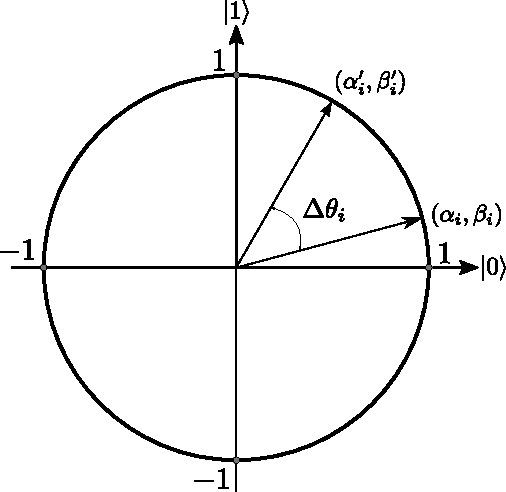
\includegraphics[width=0.45\textwidth]{rotation-gate.pdf}
    \caption{Kvantové rotační hradlo. Obrázek byl převzat s úpravami z~\cite{NaturalComputing}.}
    \label{fig:rotation-gate}
\end{figure}
Unitární vlastnost rotačního hradla zaručuje, že součet pravděpodobností bitového stavu $0$ a~$1$ po pozorování zůstává roven $1$. 
Výsledný stav qubitu se tedy po aplikaci hradla vždy nachází na jednotkové kružnici, vizte obrázek~\ref{fig:rotation-gate}~\cite{NaturalComputing}.

Aby mutace postupně přizpůsobovala hodnoty kvantového chromozomu směrem k nejlepšímu nalezenému jedinci v aktuální pozorované populaci, lze využít různé přístupy. 
Jeden z možných způsobů spočívá ve využití tabulky~\ref{tab:look-up-table-Delta}, kde postup pro výběr hodnoty parametru $\Delta\theta_i$ je následující~\cite{NaturalComputing}:
\begin{enumerate}
    \item Pomocí aktuálního kvantového chromozomu $q = \begin{pmatrix} q_1 & q_2 & \dots & q_m \end{pmatrix}$ složeného z kvantových bitů $ q_i = \left[ \alpha_i, \beta_i \right]^\text{T}$ pro $i=1,2,\,\dots\,,m$, respektive
        \begin{equation*}
            q =
            \begin{bmatrix}
                \alpha_1 & \alpha_2 & \dots & \alpha_m \\
                \beta_1  & \beta_2  & \dots & \beta_m
            \end{bmatrix},
        \end{equation*}
        je vytvořen binární chromozom $x = \begin{pmatrix} x_1 & x_2 & \dots & x_m \end{pmatrix}$.
        Hodnota $x_i$ je určena na základě qubitu $q_i$, respektive jeho parametru $\alpha_i$, následujícím způsobem:
        \begin{equation*}
            x_i =
            \begin{cases} 
                0 & \text{pokud } \alpha_i^2 \leq 0{,}5, \\
                1 & \text{jinak}.
            \end{cases}
        \end{equation*}
    \item Z populace je vybráno nejlepší binární řešení $b = \begin{pmatrix} b_1 & b_2 & \dots & b_m \end{pmatrix}$.
    \item Na základě hodnot $x_i$ a $b_i$ je z vyhledávací tabulky~\ref{tab:look-up-table-Delta} vybrána hodnota $\Delta\theta_i$ následovně:
        \begin{table}[ht!]
            \centering
            \begin{tabular}{|c c|c|}
            \hline
            $x_i$ & $b_i$ & $\Delta\theta_i$ \\
            \hline
            1     & 1     & 0                \\ 
            0     & 1     & $\delta$              \\ 
            0     & 0     & 0                \\ 
            1     & 0     & $-\delta$             \\
            \hline
            \end{tabular}
            \caption{Vyhledávací tabulka pro parametr $\Delta\theta_i$.}
            \label{tab:look-up-table-Delta}
        \end{table}
        \begin{itemize}
            \item Pokud $x_i = b_i$, pak $\Delta\theta_i = 0$, respektive parametry $\alpha_i$ a $\beta_i$ qubitu $q_i$ zůstanou zachovány.
            \item Pokud $x_i = 1\,\wedge\,b_i = 0$, pak $\Delta\theta_i = -\delta$, respektive dojde ke snížení pravděpodobnosti pozorování binární hodnoty 1 na pozici $i$ chromozomu $q$. 
            \item Pokud $x_i = 0\,\wedge\,b_i = 1$, pak $\Delta\theta_i =  \delta$, respektive dojde ke zvýšení pravděpodobnosti pozorování binární hodnoty 1 na pozici $i$ chromozomu $q$. 
        \end{itemize}
        Tabulka~\ref{tab:look-up-table-Delta} nebere v úvahu kvadranty z obrázku~\ref{fig:rotation-gate}, v nichž koeficienty $\alpha_i$ nebo $\beta_i$ mohou být záporné, tudíž je možné upravit rovnici~\ref{eq:rotation-gate-angles} tak, aby aktualizovala $i$-tý kvantový bit $\begin{bmatrix} \alpha_i \\ \beta_i \end{bmatrix}$ následovně:
        \begin{equation}\label{eq:rotation-gate-angles-update}
            \begin{bmatrix}
                \alpha_i' \\
                \beta_i' 
            \end{bmatrix}
            =
            R\left(\xi \left( \Delta\theta_i \right)\right) \cdot
            \begin{bmatrix}
                \alpha_i \\
                \beta_i 
            \end{bmatrix},
        \end{equation}
        kde $\xi \left( \Delta\theta_i \right) = s\left( \alpha_i , \beta_i \right) \cdot \Delta\theta_i $, přičemž $s\left( \alpha_i , \beta_i \right)$ a $\Delta\theta_i$ určují směr rotace a úhel, vizte vyhledávací tabulku~\ref{tab:look-up-table-angle-update}.
        \begin{table}[ht!]
            \centering
            \begin{tabular}{|c|c|c|c|c|c|c|c|}
                \hline
                $x_i$ & $b_i$ & $f\left(x\right) > f\left(b\right)$ & $\Delta \theta_i$ & \multicolumn{4}{c|}{$s\left(\alpha_i, \beta_i\right)$} \\
                \cline{5-8}
                & & & & $\alpha_i \beta_i > 0$& $\alpha_i \beta_i < 0$ & $ \alpha_i = 0$ & $\beta_i = 0$ \\
                \hline
                0 & 0 & Nepravda & $0$      & $0$  & $0$  & $0$     & $0$ \\
                0 & 0 & Pravda   & $0$      & $0$  & $0$  & $0$     & $0$ \\
                0 & 1 & Nepravda & $\delta$ & $+1$ & $-1$ & $0$     & $\pm 1$ \\
                0 & 1 & Pravda   & $\delta$ & $-1$ & $+1$ & $\pm 1$ & $0$ \\
                1 & 0 & Nepravda & $\delta$ & $-1$ & $+1$ & $\pm 1$ & $0$ \\
                1 & 0 & Pravda   & $\delta$ & $+1$ & $-1$ & $0$     & $\pm 1$ \\
                1 & 1 & Nepravda & $0$      & $0$  & $0$  & $0$     & $0$ \\
                1 & 1 & Pravda   & $0$      & $0$  & $0$  & $0$     & $0$ \\
                \hline
            \end{tabular}
            \caption{Vyhledávací tabulka pro parametr $\Delta\theta_i$ a $s\left(\alpha_i, \beta_i\right)$, kde je parametr $\delta$ obvykle nastaven na malou hodnotu (běžně $0.01 \pi$).}
            \label{tab:look-up-table-angle-update}
        \end{table}
\end{enumerate}

V kvantově inspirovaných evolučních algoritmech se v současné době nevyužívají komplexní koeficienty z kvantové mechaniky, ale výlučně se používají reálné koeficienty, což vede na reprezentaci kvantového stavu pomocí jednotkové kružnice namísto Blochovy sféry, jak je zřejmé z obrázku~\ref{fig:rotation-gate}~\cite{NaturalComputing}.

\subsection{Kvantová mutace}\label{subsec:quantum-mutation}
Kvantová mutace je inspirována mutací ze standardních evolučních algoritmů v podobě~\cite{NaturalComputing}:
\begin{equation*}
    Q^*\left(t\right) = a \cdot B_{\text{best}}\left(t\right) + (1 - a) \cdot (1 - B_{\text{best}}\left(t\right))
\end{equation*}
\begin{equation*}
    Q\left(t+1\right) = Q^*\left(t\right) + b \cdot r,
\end{equation*}
kde
\begin{itemize}
    \item $B_{\text{best}}\left(t\right)$ reprezentuje nejlepší nalezené řešení v iteraci $t$,
    \item $Q^*\left(t\right)$ je dočasný kvantový chromozom,
    \item $r$ je náhodné číslo pocházející z normálního rozdělení $N\left(0,1\right)$,
    \item $a$ a $b$ jsou parametry řídící poměr průzkumu a exploatace.
\end{itemize}

Případně existují i další možné metody pro mutaci kvantového chromozomu~\cite{NaturalComputing}.

\section{Kvantově inspirovaný genetický algoritmus}\label{sec:qiga}
Kanonický příklad kvantově inspirovaného genetického algoritmu (\emph{Quantum Inspired Genetic Algorithm\,--\,QIGA}), jenž je principiálně podobný ostatním evolučním algoritmům, je popsán algoritmem~\ref{alg:BinaryQIEA}, kde parametr $t_{\text{max}}$ udává maximální počet iterací (generací) algoritmu a parametr $t$ označuje aktuálně prováděnou iteraci~\cite{NaturalComputing}. 

\begin{algorithm}[ht]
    \caption{Kvantově inspirovaný genetický algoritmus~\cite{NaturalComputing}}
    \label{alg:BinaryQIEA}
    $t \gets 0$\;
    Inicializace populace $Q\left(t\right)$ kvantových chromozomů\;
    Vytvoření množiny řešení $P\left(t\right)$ pozorováním $Q\left(t\right)$\;
    Ohodnocení $P\left(t\right)$ a vybrání nejlepšího řešení z populace\;
    Uložení nejlepšího řešení do $B\left(t\right)$\;
    \While{$t < t_{\text{max}}$}{
        $t \gets t + 1$\;
        Vytvoření $P\left(t\right)$ pozorováním $Q\left(t-1\right)$\;
        Ohodnocení populace $P\left(t\right)$\;
        \uIf{\emph{Nejlepší řešení z} $P\left(t\right)$ > $B\left(t-1\right)$}{
            Uložení nejlepších řešení z $P\left(t\right)$ do $B\left(t\right)$\;
        }
        \Else{
            Uložení $B\left(t-1\right)$ do $B\left(t\right)$\;
        }
        Vytvoření $Q\left(t\right)$ pomocí $B\left(t\right)$\;
    }
\end{algorithm}

Uvažujme počáteční generaci $t=0$, kdy algoritmus začíná inicializací počáteční populace $Q\left(t\right)$ čítající $n$ kvantových chromozomů:
\begin{equation}\label{eq:q(t)}
    Q\left(t\right) = \left\{ q_1\left(t\right), q_2\left(t\right),\,\dots\,, q_n\left(t\right) \right\},
\end{equation}
přičemž každý z chromozomů $q_j\left(t\right)$ pro $j = 1,2,\,\dots\,,n$ je tvořen $m$ kvantovými bity $\psi_{j_i}\left(t\right)$ složenými z koeficientů $\alpha$~a~$\beta$ jako:
\begin{equation*}
    q_j\left(t\right) =
    \begin{bmatrix}
        \psi_{j_1}\left(t\right) & \psi_{j_2}\left(t\right) & \dots & \psi_{j_m}\left(t\right) \\
    \end{bmatrix}
    =
    \begin{bmatrix}
        \alpha_{j_1}\left(t\right) & \alpha_{j_2}\left(t\right) & \dots & \alpha_{j_m}\left(t\right) \\
        \beta_{j_1}\left(t\right)  & \beta_{j_2}\left(t\right)  & \dots & \alpha_{j_m}\left(t\right)
    \end{bmatrix},
\end{equation*}
kde jsou koeficienty $\alpha_{j_i}\left(t\right)$ a $\beta_{j_i}\left(t\right)$ pro $i = 1,2,\,\dots\,,m$ v každém kvantovém bitu $q_j\left(t\right)$ nastaveny na běžně používanou hodnotu $\frac{1}{\sqrt{2}}$. 
Respektive počáteční pravděpodobnost výsledného stavu 0 nebo 1 je po provedeném pozorování rovna $\left(\frac{1}{\sqrt{2}}\right)^2 = 0{,}5$. 
Případně mohou být koeficienty $\alpha$ a $\beta$ nastaveny na libovolné hodnoty, které lépe vyhovují řešenému problému, avšak stále musí splňovat podmínku normalizace danou rovnicí~\ref{eq:a2+b2=1}~\cite{NaturalComputing,qiga}. 

Nad vytvořenou počáteční populací $Q\left(t\right)$ může být provedeno pozorování, čímž dojde k vygenerování množiny řešení:
\begin{equation}\label{eq:p(t)}
    P\left(t\right) = \left\{ p_1\left(t\right), p_2\left(t\right), \dots, p_n\left(t\right) \right\},
\end{equation}
kde je každé řešení $p_j$ pro $j = 1, 2,\,\dots\,, n$ reprezentováno binárním řetězcem složeného z~$m$~bitů:
\begin{equation*}
    p_j\left(t\right) = 
    \begin{pmatrix}
        x_{j_1}\left(t\right) & x_{j_2}\left(t\right) & \dots & x_{j_m}\left(t\right)
    \end{pmatrix}.
\end{equation*}
Při jedné z možných metod generování množiny řešení $P\left(t\right)$ je na $i$-té pozici $j$-tého bitu $x_{j_{i}}$ nastavena hodnota $1$ v případě, že náhodně vygenerované číslo $r_i \in \langle 0, 1\rangle$ splňuje podmínku~$r_i > \left| \alpha_i\left(t\right) \right|^2$, jinak je na tuto pozici nastavena hodnota $0$~\cite{NaturalComputing,qiga}.

Vygenerování množiny řešení $P\left(t\right)$ může být provedeno několika způsoby~\cite{NaturalComputing}:
\begin{itemize}
    \item Použitím jednoho kvantového chromozomu, kdy je množina řešení $P\left(t\right)$ vygenerována pomocí $n$-násobného pozorování tohoto jediného chromozomu. 
    \item Použitím malé populace kvantových chromozomů, kdy je každý z nich pozorován tolikrát, aby celkový počet pozorování odpovídal velikosti výsledné množiny řešení $P\left(t\right)$.
    \item Použitím stejného počtu kvantových chromozomů jako je velikost populace $P\left(t\right)$.
\end{itemize}

Posléze je každé binární řešení $p_j\left(t\right)$ ohodnoceno fitness funkcí. 
Nejlepší řešení $p_k\left(t\right)$ je vybráno na základě tohoto ohodnocení a použito k určení aktuálně nejlepšího řešení:
\begin{equation*}
    B\left(t\right) =
    \begin{pmatrix}
        b_1\left(t\right) & b_2\left(t\right) & \dots & b_m\left(t\right)
    \end{pmatrix},
\end{equation*}
kde $b_i\left(t\right) = x_{k_i}\left(t\right)$ pro $i = 1,2,\,\dots\,,m$~\cite{NaturalComputing,qiga}.

Uvažujme generaci $t$ pro $t>0\,\wedge\,t<t_{\text{max}}$ v rámci smyčky \emph{QIGA}. 
V iteraci $t$ je vytvořena množina řešení $P\left(t\right)$ pozorováním předchozí populace $Q\left(t-1\right)$, jenž je následně ohodnocena fitness funkcí. 
Nejlepší řešení napříč $P\left(t\right)$ a $B\left(t-1\right)$ je uloženo do $B\left(t\right)$. 
Hlavní částí smyčky algoritmu je vytvoření populace $Q\left(t\right)$ na základě $B\left(t\right)$ s cílem její evoluce, která může být provedena několika způsoby a to například~\cite{NaturalComputing}:
\begin{itemize}
    \item použitím některé z variant kvantové mutace, vizte podsekci~\ref{subsec:quantum-mutation}, nebo
    \item aplikací kvantových rotačních hradel, vizte podsekci~\ref{subsec:quantum-gates} a popis níže.
\end{itemize}

Uvažujme $i$-tý kvantový bit $\psi_{j_i}\left(t-1\right) = \begin{bmatrix} \alpha_{j_i}\left(t-1\right) \\ \beta_{j_i}\left(t-1\right) \end{bmatrix}$ $j$-tého jedince. 
Nová hodnota kvantového bitu $\psi_{j_i}\left(t\right)$ je spočtena pomocí kvantového rotačního hradla $R\left(\right)$ následujícím způsobem:
\begin{equation*}\label{eq:qiga-rotation-gate-angles}
    \psi_{j_i}\left(t\right) =
    \begin{bmatrix}
        \alpha_{j_i}\left(t\right) \\
        \beta_{j_i}\left(t\right)
    \end{bmatrix}
    =
    R\left(\Delta\theta_{j_i}\right) \cdot
    \begin{bmatrix}
        \alpha_{j_i}\left(t-1\right) \\
        \beta_{j_i}\left(t-1\right) 
    \end{bmatrix},
\end{equation*}
kde $\alpha_{j_i}\left(t\right)$ a $\beta_{j_i}\left(t\right)$ jsou nové pravděpodobnostní koeficienty aktualizovaného kvantového bitu. Proces je znázorněn na obrázku~\ref{fig:qiga-rotation-gate}.

\begin{figure}[ht!]
    \centering
    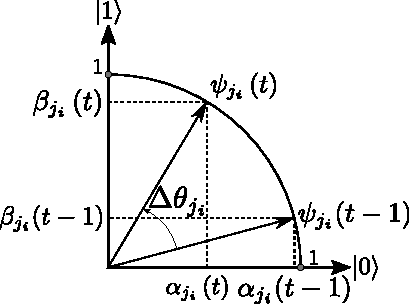
\includegraphics[width=0.5\textwidth]{qiga-rotation-gate.pdf}
    \caption{Znázornění principu kvantové rotace, kde je rotací o úhel $\Delta\theta_{j_i}$ počáteční stav $\psi_{j_i}\left(t-1\right) = \begin{bmatrix} \alpha_{j_i}\left(t-1\right) \\ \beta_{j_i}\left(t-1\right) \end{bmatrix}$ aktualizován na nový stav $\psi_{j_i}\left(t\right) = \begin{bmatrix} \alpha_{j_i}\left(t\right) \\ \beta_{j_i}\left(t\right) \end{bmatrix}$. Obrázek převzat s~úpravami z~\cite{qisa}.}
    \label{fig:qiga-rotation-gate}
\end{figure}

Kvantové chromozomy jsou v tomto aktualizačním kroku upraveny tak, aby v následující generaci docházelo k pravděpodobnějšímu generování dosud nejlepšího nalezeného řešení. 
Iterace evolučního procesu se opakují, dokud není splněna ukončující podmínka, přičemž se algoritmus postupně blíží k nejlepšímu nalezenému řešení, jednotlivé qubity kvantového chromozomu konvergují k hodnotě 0 nebo 1~\cite{NaturalComputing,qiga}.

\section{Kvantově inspirované simulované žíhání}\label{sec:qisa}
Tato sekce se zaměří na představení kvantově inspirovaného simulovaného žíhání (\emph{Quantum Inspired Simulated Annealing\,--\,QISA}), což je algoritmus, jenž kombinuje principy klasického simulovaného žíhání (\emph{Simulated Annealing\,--\,SA}) a kvantového počítání. 
Algoritmus \emph{QISA}, znázorněný algoritmem~\ref{alg:qisa}, vychází principiálně z algoritmu \emph{QIGA} ze sekce~\ref{sec:qiga}, jenž je rozšířen o principy \emph{SA} a jehož klasické pozorování kvantové populace je upraveno na tepelně-řízené pozorování (\emph{heated observation}). 
Obdobně jako v pseudokódu algoritmu~\ref{alg:BinaryQIEA}~\emph{QIGA} proměnná $t$ reprezentuje aktuálně prováděnou iteraci a hodnota $t_{\text{max}}$ určuje maximální počet generací evolučního procesu~\cite{qisa}. 

\begin{algorithm}[ht]
    \caption{Kvantově inspirované simulované žíhání~\cite{qisa}}
    \label{alg:qisa}
    Inicializace počáteční teploty $T_0$\;
    Selekce chladicího plánu\;
    $t \gets 0$\;
    Inicializace populace $Q\left(t\right)$ kvantových chromozomů\;
    Vytvoření množiny řešení $P\left(t\right)$ tepelně-řízeným pozorováním $Q\left(t\right)$\;
    Získání energie $E\left(t\right)$ populace $P\left(t\right)$\;
    \While{$t < t_{\text{max}}$}{
        $t \gets t + 1$\;
        Vytvoření množiny řešení $P\left(t\right)$ tepelně-řízeným pozorováním $Q\left(t-1\right)$\;
        Získání energie $E_P\left(t\right)$ množiny řešení $P\left(t\right)$\;
        \uIf{$E_P\left(t\right) \leq E\left(t-1\right)$}{
            Vytvoření $Q\left(t\right)$ na základě $\begin{bmatrix} 1 - P\left(t\right) \\ P\left(t\right) \end{bmatrix}$\;
            Vytvoření $E\left(t\right)$ na základě $E_P\left(t\right)$\;
        }
        \Else{
            Vytvoření $Q\left(t\right)$ na základě $R_Q\left(Q\left(t-1\right),P\left(t\right)\right)$\;
            Vytvoření $E\left(t\right)$ na základě $U_E\left(E\left(t-1\right),E_P\left(t\right)\right)$\;
        }
        Aktualizace $T_t$ pomocí chladicího plánu\;
    }
\end{algorithm}

Na začátku algoritmu je inicializována počáteční teplota $T_0$ pomocí standardní odchylky následovně:
\begin{equation}\label{eq:qisa-T0}
    T_0 = \sigma = \sqrt{\frac{1}{N}\sum_{i=1}^{N}\left(x_i - \bar{x}\right)^2},
\end{equation}
kde
\begin{itemize}
    \item $x_i$ je $i$-té náhodně vygenerované řešení,
    \item $\bar{x}$ je průměr vygenerovaných řešení a
    \item $N$ je počet vygenerovaných řešení.
\end{itemize}
Tato inicializace teploty $T_0$ je vhodná pro řešení numerických optimalizačních problémů, kde jsou řešením reálné hodnoty, přičemž se standardně při výpočtu počáteční teploty uvažuje 1000 náhodně vygenerovaných řešení, respektive $N=1000$~\cite{qisa,FundamentalsOfProbability}.

Následuje výběr chladicího plánu. Příkladem takového plánu je exponenciální chladicí plán, jenž je definován jako:
\begin{equation*}
    T\left(t\right) = T_0 \cdot a^t,
\end{equation*}
kde $T_0$ je počáteční teplota, $a$ je chladicí koeficient a $t$ je chladicí krok (iterace)~\cite{qisa}. 

Uvažujme $t= 0$. Po výpočtu počáteční teploty $T_0$ a výběru chladicího plánu je vygenerována počáteční populace $Q\left(t\right)$, vizte rovnici~\ref{eq:q(t)}, jež je pozorována pomocí tepelně-řízeného pozorování. 
Nechť $q_j\left(t\right)$ je aktuálně pozorovaný kvantový chromozom, pak jsou pravděpodobnosti pozorování binárních stavů $i$-tého kvantového bitu dány jako~\cite{qisa}:
\begin{eqnarray*}
    \left|\alpha_{j_i}^h\left(t\right)\right|^2 &=& \left|\alpha_{j_i}\left(t\right)\right|^2 + \left(0,5 - \left|\alpha_{j_i}\left(t\right)\right|^2\right) \cdot h\left(T_t\right) \\
    \left|\beta_{j_i}^h\left(t\right) \right|^2 &=& \left|\beta_{j_i}\left(t\right) \right|^2 + \left(0,5 - \left|\beta_{j_i}\left(t\right) \right|^2\right) \cdot h\left(T_t\right),
\end{eqnarray*}
kde 
\begin{itemize}
    \item $\left|\alpha_{j_i}^h\left(t\right)\right|^2$ je pravděpodobnost pozorování stavu 0,
    \item $\left|\beta_{j_i}^h\left(t\right)\right|^2$ je pravděpodobnost pozorování stavu 1 a
    \item $h\left(T_t\right)$ pro $0 \leq h\left(T_t\right) \leq 1$ je zahřívací funkce (\emph{heating function}). 
\end{itemize}

Na rozdíl od klasického pozorování, kde je náhodně vygenerovaná hodnota $r_i$ porovnávána s~$\left|\alpha_{j_i}\left(t\right) \right|^2$ nebo s $\left|\beta_{j_i}\left(t\right) \right|^2$, u tepelně-řízeného pozorování se porovnává hodnota $r_i$~s~$\left|\alpha_{j_i}^h\left(t\right) \right|^2$ nebo s $\left|\beta_{j_i}^h\left(t\right) \right|^2$. 
Tyto pravděpodobnosti vycházejí z klasických koeficientů kvantového bitu, jež jsou navíc upraveny tepelným procesem. 
Tento proces zajišťuje vyrovnání pravděpodobností pro pozorování stavu 0 a 1 u každého kvantového bitu, čímž nedochází k rychlé konvergenci k~jednomu stavu a tudíž nejsou jednotlivé kvantové bity vázány na jeden konkrétní stav. 
Síla tohoto zahřívání určuje, jak moc budou pozorované bity závislé na konkrétním stavu, respektive když $h\left(T\right) = 0$, jsou pozorované kvantové bity zcela určeny aktuálním řešením, zatímco když $h\left(T\right) = 1$, je výsledek pozorování zcela náhodný~\cite{qisa}. 

Uvažujme dvě zahřívací metody. První z nich se nazývá konstantní zahřívání a má tvar:
\begin{equation}\label{eq:qisa-const}
    h\left(T\right) = w,
\end{equation}
kde $w$ je konstanta. Druhá metoda je tzv. sigmoidní funkce, která má tvar:
\begin{equation}\label{eq:qisa-sigmo}
    h\left(T\right) = \frac{w_3}{1 + e^{-w_1 \left(\frac{T}{T_0} - w_2 \right)}} + w_4,
\end{equation}
kde $w_1$, $w_2$, $w_3$ a $w_4$ jsou kladné kontrolní parametry a $T_0$ je počáteční teplota. 
Princip sigmoidního zahřívání spočívá v tom, že při vyšších teplotách je zahřívání silnější, zatímco při nižších teplotách je slabší, což znamená, že na počátku evoluce bude mít pozorované řešení větší závislost na aktuálním kvantovém bitu, což pomáhá globálnímu prohledávání. 
Naopak na konci evoluce bude závislost menší, a tudíž se prohledávání více zaměří na lokální oblasti~\cite{qisa}. 

Po prvním provedeném pozorování je z počáteční množiny řešení $P\left(t\right)$, vizte rovnici~\ref{eq:p(t)}, získána prvotní energie řešení ve tvaru:
\begin{equation*}
    E\left(t\right) = \left\{ e_1\left(t\right), e_2\left(t\right),\,\dots\,, e_n\left(t\right) \right\},
\end{equation*}
kde $e_j \left( t \right) = f\left( p_j \left( t \right) \right)$ pro $j = 1,2,\,\dots\,n$, přičemž $p_j\left( t \right)$ je řešení získané tepelně-řízeným pozorováním a $f\left( \right)$ je fitness funkce~\cite{qisa}.

Uvažujme generaci $t$ pro $t>0\,\wedge\,t < t_{\text{max}}$ v rámci smyčky \emph{QISA}. 
V iteraci $t$ je vytvořena množina řešení $P\left(t\right)$ tepelně-řízeným pozorováním populace $Q\left(t-1\right)$, ze které je následně získána energie $E_P\left(t\right)$~\cite{qisa}.

Pokud je splněna akceptační podmínka
\begin{equation}\label{eq:qisa-if}
    e^P_j\left(t\right) \leq e_j\left(t-1\right),
\end{equation}
kde $j = 1,2,\,\dots\,,n$ pak:
\begin{itemize}
    \item je vytvořena kvantové populace $Q\left(t\right)$ jedinců jako $\psi_{j_i}\left(t\right) = \begin{bmatrix} 1 - x_{j_i}\left(t-1\right) \\ x_{j_i}\left(t-1\right) \end{bmatrix}$ pro $i=1,2,\,\dots\,,m$, vizte obrázek~\ref{fig:rotation-gate-a}, a následně
    \item je vytvořena energie $E\left(t\right)$ jako $e_j\left(t\right) = e_j\left(t-1\right)$.
\end{itemize}
jinak
\begin{itemize}
    \item je vytvořena kvantové populace $Q\left(t\right)$ pomocí $R_Q\left(Q\left(t-1\right), P\left(t\right) \right)$, vizte obrázek~\ref{fig:rotation-gate-b}, a následně
    \item je vytvořena energie $E\left(t\right)$ jako $U_E\left(E\left(t-1\right), E_P\left(t\right)\right)$,
\end{itemize}
kde $R_Q\left(\right)$ je rotační funkce, vizte podsekci~\ref{subsec:qisa-rot}, a $U_E\left(\right)$ je funkce pro aktualizaci energie, vizte podsekci~\ref{subsec:qisa-upd}.
Po provedené aktualizaci kvantové populace a energie je aktualizována teplota $T_t$ v závislosti na vybraném chladicím plánu. 
Iterace evolučního procesu \emph{QISA} jsou opakovány, dokud není splněna ukončující podmínka~\cite{qisa}.
\begin{figure}[ht!]
    \centering
    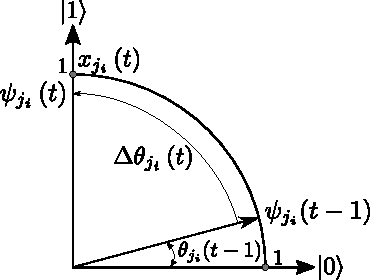
\includegraphics[width=0.5\textwidth]{qisa-rotation-gate-a.pdf}
    \caption{Pokud $e^P_j\left(t\right) \leq e_j\left(t-1\right)$ pro $j = 1,2,\,\dots\,,n$, kde uvažujme $i$-tý kvantový bit $\psi_{j_i}\left(t-1\right)$ $j$-tého jedince a binární hodnotu $x_{j_i} \left(t\right)$, pak je kvantový bitu $\psi_{j_i}\left(t\right)$ nastaven na novou hodnotu $\begin{bmatrix} 1 - x_{j_i}\left(t\right) \\ x_{j_i}\left(t\right) \end{bmatrix}$. Obrázek převzat s úpravami z~\cite{qisa}.}
    \label{fig:rotation-gate-a}
\end{figure}

\begin{figure}[ht!]
    \centering
    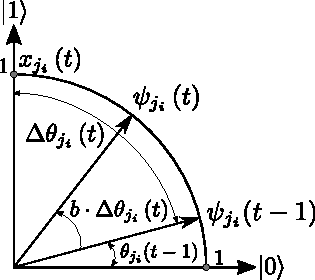
\includegraphics[width=0.42\textwidth]{qisa-rotation-gate-b.pdf}
    \caption{Pokud $e^P_j\left(t\right) > e_j\left(t-1\right)$ pro $j = 1,2,\,\dots\,,n$, kde uvažujme $i$-tý kvantový bit $\psi_{j_i}\left(t-1\right)$ $j$-tého jedince a binární hodnotu $x_{j_i} \left(t\right)$, pak je nový kvantový bit $\psi_{j_i}\left(t\right)$ získán aktualizací koeficientů o úhel $b \cdot \Delta\theta_{j_i}\left(t\right)$ směrem k~$x_{j_i}\left(t\right)$ pomocí kvantového rotačního hradla. Obrázek převzat s úpravami z~\cite{qisa}.}
    \label{fig:rotation-gate-b}
\end{figure}

\newpage
\subsection{Rotační funkce}\label{subsec:qisa-rot}
Rotační funkce $R_Q\left(\right)$ odpovídá kvantovému rotačnímu hradlu, vizte podsekci~\ref{subsec:quantum-gates}. 
Uvažujme $i$-tý kvantový bit $\psi_{j_i}\left(t-1\right) = \begin{bmatrix} \alpha_{j_i}\left(t-1\right) \\ \beta_{j_i}\left(t-1\right) \end{bmatrix}$ $j$-tého jedince $q_j\left(t-1\right)$ kvantové populace $Q\left(t-1\right)$. 
Nechť $\Delta\theta_{j_i}\left(t\right)$ je úhel mezi $\psi_{j_i}\left(t-1\right)$ a $x_{j_i}\left(t\right)$, pak jsou koeficienty $\psi_{j_i}\left(t-1\right)$ upraveny pomocí kvantového rotačního hradla o úhel $b \cdot \Delta\theta_{j_i}\left(t\right)$ směrem k~$x_{j_i}\left(t\right)$.
Faktor $b$ splňující $0 \leq b \leq 1$ je definován jako:
\begin{equation}\label{eq:b-factor}
    b = e^{\left(\frac{e_j\left(t-1\right) - e^P_j\left(t\right)}{T_t}\right)}, 
\end{equation}
kde $e^P_j\left(t\right)$ je energie $j$-tého prvku množiny řešení $P\left(t\right)$ a $T_t$ je aktuální teplota. Výsledný úhel $\Delta\theta_j\left(t\right)$ pro rotaci je spočten podle vzorce:
\begin{equation*}
        \Delta_{j_i}\left(t\right) = b \cdot \Delta\theta_{j_i}\left(t\right) = b \cdot \left(\frac{\pi}{2}\cdot p_{j_i}\left(t\right) - \theta_{j_i}\left(t-1\right)\right),
\end{equation*}
kde $\theta_{j_i}\left(t-1\right) = \arctan{\left(\frac{\beta_{j_i}\left(t-1\right)}{\alpha_{j_i}\left(t-1\right)}\right)}$. 
Spočítaný úhel je následně aplikován na kvantové rotační hradlo $R\left(\right)$:
\begin{equation*}
    \begin{bmatrix}
        \alpha_{j_i}\left(t\right) \\
        \beta_{j_i}\left(t\right)
    \end{bmatrix}
    =
    R\left(\Delta_{j_i}\left(t\right)\right)
    \begin{bmatrix}
        \alpha_{j_i}\left(t-1\right) \\
        \beta_{j_i}\left(t-1\right) 
    \end{bmatrix},
\end{equation*}
kde $\alpha_{j_i}\left(t\right)$ a $\beta_{j_i}\left(t\right)$ jsou nové koeficienty kvantového bitu $\psi_{j_i}\left(t\right)$~\cite{qisa}.

\subsection{Funkce pro aktualizaci energie}\label{subsec:qisa-upd}
Funkce pro aktualizaci energie $U_E\left(\right)$ není nutná v případě, že platí $e^P_j\left(t\right) \leq e_j\left(t-1\right)$, jelikož je nová energie $e_j\left(t\right)$ jedince nastavena na energii $e_j\left(t-1\right)$. 
Pokud však platí $e^P_j\left(t\right) > e_j\left(t-1\right)$, měla by být energie $e_j\left(t\right)$ nastavena na hodnotu energie odpovídající novému stavu $q_j\left(t\right)$. 
Přesná energie tohoto stavu je dána jako vážený součet energií všech $2^n$ pozorovaných stavů jedince, a to následovně:
\begin{equation*}
    E_Q = \sum_{i=0}^{2^n-1} p_i \cdot e_{j_i}
\end{equation*}
kde 
\begin{itemize}
    \item $e_{j_i}$ je energie $i$-tého pozorovaného stavu $j$-tého jedince a
    \item $p_i$ je pravděpodobnost s jakou je pozorován $i$-tý stav,
\end{itemize}
Tento výpočet je pro klasické výpočetní systémy náročný, neboť jeho výpočetní složitost roste exponenciálně s počtem kvantových bitů. 
Proto se pro výpočet energie nového řešení využívá aproximace, která je vyjádřena následující rovnicí:
\begin{equation*}
    e_j\left(t\right) = U_E\left(e_j\left(t-1\right), e^P_j\left(t\right)\right) = \cos^2{\left(b \cdot \frac{\pi}{2}\right)} \cdot e_j\left(t-1\right) + \sin^2{\left(b \cdot \frac{\pi}{2}\right)} \cdot e^P_j\left(t\right),
\end{equation*}
kde $b$ je faktor definován rovnicí~\ref{eq:b-factor}. 
Přestože tato aproximace není zcela přesná, poskytuje efektivní způsob, jak algoritmu umožnit opustit lokální optima~\cite{qisa}. 

\section{Kvantová evoluce roje}\label{sec:qse}
Tato sekce pojednává o kvantové evoluci roje (\emph{Quantum Swarm Evolutionary\,--\,QSE}), což je algoritmus kombinující principy kvantového počítání a částicového systému (\emph{Particle Swarm Optimization}) a jež je znázorněn na algoritmu~\ref{alg:qse}. 
Obdobně jako u algoritmů \emph{QIGA} a \emph{QISA}, proměnná $t$ reprezentuje aktuální iteraci a hodnota $t_{\text{max}}$ určuje maximální počet iterací evolučního procesu.

\begin{algorithm}[ht]
    \caption{Kvantová evoluce roje~\cite{qse}}
    \label{alg:qse}
    $t \gets 0$\;
    Inicializace populace $Q\left(t\right)$ kvantových chromozomů\;
    Inicializace počátečních rychlostí $V\left(t\right)$\;
    Inicializace nejlepších řešení populace $B\left(t\right)$ a globálně nejlepších řešení $G\left(t\right)$\;
    \While{$t < t_{\text{max}}$}{
        $t \gets t + 1$\;
        Vytvoření množiny řešení $P\left(t\right)$ pozorováním populace $Q\left(t-1\right)$\;
        \uIf{\emph{Nejlepší řešení z} $P\left(t\right)$ > $B\left(t-1\right)$}{
            Uložení nejlepších řešení z $P\left(t\right)$ do $B\left(t\right)$\;
        }
        \Else{
            Uložení $B\left(t-1\right)$ do $B\left(t\right)$\;
        }
        \uIf{\emph{Nejlepší řešení z} $B\left(t\right)$ > $G\left(t-1\right)$}{
            Uložení nejlepšího řešení z $B\left(t\right)$ do $G\left(t\right)$\;
        }
        \Else{
            Uložení $G\left(t-1\right)$ do $G\left(t\right)$\;
        }
        Vytvoření $V\left(t\right)$ pomocí $B\left(t\right)$ a $G\left(t\right)$\;
        Vytvoření $Q\left(t\right)$ pomocí $V\left(t\right)$\;
    }
\end{algorithm}

Na počátku algoritmu, kdy $t=0$, je inicializována počáteční populace $Q\left(t\right)$, která je složena z~$n$~kvantových chromozomů, jež jsou reprezentovány tzv. kvantovými úhly \emph{(quantum angles)} místo dříve používaných pravděpodobnostních koeficientů $\alpha$ a $\beta$, a to následovně:
\begin{equation*}
    Q\left(t\right) = \left\{q_1\left(t\right), q_2\left(t\right),\,\dots\,,q_n\left(t\right)\right\},
\end{equation*}
kde je každý z kvantových chromozomů $q_j\left(t\right)$ pro $j=1,2,\,\dots\,n$ tvořen $m$ kvantovými úhly $\varphi_{j_i}\left(t\right)$ jako:
\begin{equation*}
    q_j\left(t\right) = \begin{bmatrix} \varphi_{j_1}\left(t\right) & \varphi_{j_2}\left(t\right) & \dots & \varphi_{j_n}\left(t\right) \end{bmatrix},
\end{equation*}
jejichž hodnota je nastavena na $\frac{\pi}{4}$.
Současně dochází také k inicializaci počátečních rychlostí pro každý kvantový chromozom:
\begin{equation*}
    V\left(t\right) = \left\{ v_1\left(t\right), v_2\left(t\right) ,\,\dots\,, v_n\left(t\right)\right\},
\end{equation*}
kde je vektor rychlosti $v_j\left(t\right)$ jedince pro $j=1,2,\,\dots\,n$ definován jako:
\begin{equation*}
    v_j\left(t\right) = \begin{pmatrix} y_{j_1}\left(t\right) & y_{j_2}\left(t\right) & \dots & y_{j_m}\left(t\right) \end{pmatrix},
\end{equation*}
kde je každá rychlost $y_{j_i}$ pro $i=1,2,\,\dots\,m$ nastavena na předem danou hodnotu~\cite{qse}.

Uvažujme generaci $t>0 \wedge t<t_{\text{max}}$. Z populace $Q\left(t-1\right)$ je za pomoci pozorovací funkce $\zeta\left(\right)$ vygenerována množina řešení $P\left(t\right)$ jako
\begin{equation}
    P\left(t\right) = \left\{\zeta\left(q_1\left(t-1\right)\right), \zeta\left(q_2\left(t-1\right)\right), \,\dots\, , \zeta\left(q_n\left(t-1\right)\right) \right\} = \left\{ p_1\left(t\right), p_2\left(t\right), \dots, p_n\left(t\right) \right\},
\end{equation}
kde každé $p_j\left(t\right)$ pro $j=1,2,\,\dots\,n$ reprezentuje binární řešení problému:
\begin{equation*}
    p_j\left(t\right) = 
    \begin{pmatrix}
        x_{j_1}\left(t\right) & x_{j_2}\left(t\right) & \dots & x_{j_m}\left(t\right)
    \end{pmatrix},
\end{equation*}
kde pro každou ze složek platí:
\begin{equation*}
    x_{j_i}\left(t\right) =
    \begin{cases}
      1 & \text{je-li } r_{j_i}\left(t\right) >\cos^2 \varphi_{j_i}\left(t-1\right),\quad\text{kde}\quad r_{j_i}\left(t\right) \sim U\left(0,1\right)\\
      0 & \text{jinak.}
    \end{cases}
\end{equation*}

Jedinci ze získané množiny řešení $P\left(t\right)$ jsou ohodnoceni pomocí fitness funkce $f\left(\right)$ jako~\cite{qse}: 
\begin{equation*}
    F\left(t\right) = \left\{ f\left(p_1\left(t\right)\right), f\left(p_2\left(t\right)\right), \,\dots\,, f\left(p_n\left(t\right)\right) \right\}.
\end{equation*}
Následně je dle ohodnocení provedena aktualizace nejlepších osobních kvantových úhlů jedinců~\cite{qse}:
\begin{equation}\label{eq:pers-best}
    B_i\left(t\right) =
    \begin{cases}
        q_i\left(t\right)   & \text{je-li } f\left(p_i\left(t\right)\right) > f\left(B_i\left(t-1\right)\right), \\
        B_i\left(t-1\right) & \text{jinak.}
    \end{cases}
\end{equation}
Pro výpočet globálního nejlepšího kvantového úhlu $G\left(t\right)$ je nejprve určen index $c$ aktuálně nejlepšího osobního řešení všech jedinců jako:
\begin{equation*}
    c = \arg\max_{i=1,\dots,n} f\left(\zeta\left(B_i\left(t\right)\right)\right),\\[5pt]
\end{equation*}
jenž je využit pro aktualizaci globálního úhlu $G\left(t\right)$ jako~\cite{qse}:
\begin{equation}\label{eq:glob-best}
    G\left(t\right) =
    \begin{cases}
        B_c\left(t\right)   & \text{pokud } f\left(\zeta\left(B_c\left(t\right)\right)\right) > f\left(\zeta\left(G\left(t-1\right)\right)\right) \\
        G\left(t-1\right)   & \text{jinak.}
    \end{cases}
\end{equation}

Předposledním krokem je aktualizace rychlosti jednotlivých kvantových chromozomů pomocí vylepšeného vzorce $PSO$ algoritmu~\cite{qse}: 
\begin{equation}\label{eq:qse-velocity}
    y_{j_i}\left(t\right) = \chi \cdot
    \left( \omega \cdot y_{j_i}\left(t-1\right) 
        + c_1 \cdot r_1 \cdot \left(B_{j_i}\left(t\right) - \varphi_{j_i}\left(t-1\right) \right)
        + c_2 \cdot r_2 \cdot \left( G_{i}\left(t\right) - \varphi_{j_i}\left(t-1\right) \right)\right),
\end{equation}
kde $\chi, \omega, c_1 , c_2$ jsou koeficienty setrvačnosti a učení a $r_1,r_2\sim U\left(0,1\right)$.  

Při závěrečném kroku iterace dochází k aktualizaci kvantových úhlů jedinců v populaci následovně:
\begin{equation*}
    \varphi_{j_i}\left(t\right) = \varphi_{j_i}\left(t-1\right) + y_{j_i}\left(t\right).
\end{equation*}
Tento proces se opakuje do té doby, dokud není splněna ukončující podmínka~\cite{qse}.

\section{Kvantově inspirovaná optimalizace rojem částic}\label{sec:qipso}
Tato sekce představí algoritmus, který byl navržen v rámci práce po analýze dříve představených technik, jenž byl pojmenován jako kvantově inspirovaná optimalizaci rojem částic (\emph{Quantum Inspired Particle Swarm Optimization\,--\,QIPSO}).
Navržený algoritmus obdobně jako algoritmus \emph{QSE} využívá principy používané v \emph{PSO}. 
Hlavní rozdílem mezi algoritmem \emph{QSE} a vlastním algoritmem \emph{QIPSO} je to, že zatímco \emph{QSE} reprezentuje jedince kvantovými úhly, algoritmus \emph{QIPSO} používá dvojici pravděpodobnostních koeficientů, jenž jsou aktualizovány kvantovým rotačním hradlem, podobně jako u algoritmů \emph{QIGA} a \emph{QISA}. 
Obdobně jako u výše uvedených algoritmů proměnná $t$~označuje aktuální iteraci algoritmu a~proměnná $t_{\text{max}}$ značí maximální počet iterací. 

\begin{algorithm}[ht]
    \caption{Kvantově inspirovaná optimalizace rojem částic}
    \label{alg:qipso}
    $t \gets 0$\;
    Inicializace populace $Q\left(t\right)$ kvantových chromozomů\;
    Inicializace počátečních rychlostí $V\left(t\right)$\;
    Inicializace nejlepších řešení populace $B\left(t\right)$ a globálně nejlepších řešení $G\left(t\right)$\;
    \While{$t < t_{\text{max}}$}{
        $t \gets t + 1$\;
        Vytvoření množiny řešení $P\left(t\right)$ pozorováním populace $Q\left(t-1\right)$\;
        \uIf{\emph{Nejlepší řešení z} $P\left(t\right)$ > $B\left(t-1\right)$}{
            Uložení nejlepších řešení z $P\left(t\right)$ do $B\left(t\right)$\;
        }
        \Else{
            Uložení $B\left(t-1\right)$ do $B\left(t\right)$\;
        }
        \uIf{\emph{Nejlepší řešení z} $B\left(t\right)$ > $G\left(t-1\right)$}{
            Uložení nejlepšího řešení z $B\left(t\right)$ do $G\left(t\right)$\;
        }
        \Else{
            Uložení $G\left(t-1\right)$ do $G\left(t\right)$\;
        }
        Vytvoření $V\left(t\right)$ pomocí $B\left(t\right)$ a $G\left(t\right)$\;
        Vytvoření $Q\left(t\right)$ pomocí $V\left(t\right)$\;
    }
\end{algorithm}

Uvažujme $t=0$. Algoritmus začíná inicializací počáteční populace $Q\left(t\right)$ čítající $n$~kvantových chromozomů jako: 
\begin{equation*}
    Q\left(t\right) = \left\{q_1\left(t\right), q_2\left(t\right),\,\dots\,,q_n\left(t\right)\right\},
\end{equation*}
kde každý jedinec $q_j\left(t\right)$ pro $j=1,2,\,\dots\,n$ je složen z $m$ dvojic pravděpodobnostních koeficientů $\alpha_{j_i}\left(t\right)$ a $\beta_{j_i}\left(t\right)$ pro $i=1,2,\,\dots\,m$, jejichž hodnota je natavena na $\frac{1}{\sqrt{2}}$.
Společně s~inicializací populace je pro každého jedince $q_j\left(t\right)$ vytvořen vektor rychlostí jako:
\begin{equation*}
    v_j\left(t\right) = \begin{pmatrix} y_{j_1}\left(t\right) & y_{j_2}\left(t\right) & \dots & y_{j_m}\left(t\right) \end{pmatrix},
\end{equation*}

Uvažujme iteraci algoritmu $t>0 \wedge t<t_{\text{max}}$. 
Nejdříve je provedeno pozorování populace $Q\left(t-1\right)$, čímž vznikne množina řešení $P\left(t\right)$, která je následně ohodnocena fitness funkcí $f\left(\right)$. 
Pomocí získaného ohodnocení jsou aktualizovány nejlepší řešení jednotlivých kvantových chromozomů, vizte rovnici~\ref{eq:pers-best}, a globálně nejlepší řešení, vizte rovnici~\ref{eq:glob-best}. 

Následuje aktualizace vektorů rychlostí pomocí rovnice:
\begin{equation*}
    y_{j_i}\left(t\right) = \omega \cdot y_{j_i}\left(t-1\right) + c_1 \cdot r_1 \cdot (b_{j_i}\left(t\right) - x_{j_i}\left(t\right)) + c_2 \cdot r_2 \cdot (g_i\left(t\right) - x_{j_i}\left(t\right)),
\end{equation*}
kde $\omega$ je koeficient tření \emph{(friction)} nebo inerciální váha (\emph{intercal weight})~\cite{PSO-c1c2w} a hodnoty $c_1,c_2$ reprezentují, po řadě, vliv osobního a~globálně nejlepšího řešení. 
Koeficienty $r_1, r_2$ obdobně jako u \emph{QSE} představují náhodné proměnné. 

Následně jsou pomocí aktualizovaných rychlostí upraveny pravděpodobnostní koeficienty $\alpha_{j_i}\left(t-1\right), \beta_{j_i}\left(t-1\right)$ jednotlivých kvantových chromozomů pomocí kvantového rotačního hradla $R\left(\right)$ jako: 
\begin{equation*}
    \begin{bmatrix}
        \alpha_{j_i}\left(t\right) \\
        \beta_{j_i}\left(t\right)
    \end{bmatrix}
    =
    R\left(y_{j_i}\left(t\right)\right) \cdot
    \begin{bmatrix}
        \alpha_{j_i}\left(t-1\right) \\
        \beta_{j_i}\left(t-1\right) 
    \end{bmatrix}.
\end{equation*}
Iterace algoritmu jsou opakovány do té doby, dokud není splněna ukončující podmínka. 

\section{Aplikace kvantově inspirovaných evolučních algoritmů}
Kvantově inspirované evoluční algoritmy nacházejí uplatnění v různých oblastech strojového učení a optimalizace. 
Příkladem může být jejich využití v návrhu konvolučních neuronových sítí, kde tyto algoritmy umožňují robustně vyhledat silný klasifikátor~\cite{QIEA-CNN}. 
Kvantově inspirované evoluční algoritmy mohou být rovněž použity při optimalizaci přepojování elektrických distribučních sítí~\cite{QIEA-net}. 
Dále se například uvažuje jejich aplikace v analogově evolvovatelném hardwaru~\cite{QIEA-EHW}. 

Souhrnný přehled vybraných aplikací \emph{QIEA} v různých oblastech, od kombinatorické optimalizace po numerickou optimalizaci, společně s jejich komentářem přinášejí následující dvě studie~\cite{QIEA-survey1, QIEA-survey2}. 
Kvantově inspirované evoluční algoritmy jsou v současné době značně zkoumány a stále vznikají nové studie rozšiřující jejich praktické využití. 
